\documentclass[conference]{IEEEtran}
\IEEEoverridecommandlockouts
% The preceding line is only needed to identify funding in the first footnote. If that is unneeded, please comment it out.
\usepackage{cite}
\usepackage{amsmath,amssymb,amsfonts}
\usepackage{algorithmic}
\usepackage{graphicx}
\usepackage{textcomp}
\usepackage{xcolor}
\usepackage{caption}
\usepackage{subcaption}
\usepackage{subfiles}
\usepackage{siunitx}
\usepackage{gensymb}
\usepackage{hyperref}
\hypersetup{
    colorlinks=false,
    linkcolor=blue,
    filecolor=magenta,      
    urlcolor=cyan,
    pdftitle={Overleaf Example},
    pdfpagemode=FullScreen,
    }
    
\graphicspath{{\subfix{../images/}}}
\def\BibTeX{{\rm B\kern-.05em{\sc i\kern-.025em b}\kern-.08em
    T\kern-.1667em\lower.7ex\hbox{E}\kern-.125emX}}
\begin{document}

\title{Analysis, Prototyping and Locomotion Control of a Quadruped Robot\\
% {\footnotesize \textsuperscript{*}Note: Sub-titles are not captured in Xplore and
% should not be used}
% \thanks{Identify applicable funding agency here. If none, delete this.}
}

%TODO
\author{\IEEEauthorblockN{1\textsuperscript{st} Lucas Souza}
  \IEEEauthorblockA{\textit{Autonomous Robotics Research Center} \\
    \textit{Technology Innovation Institute}\\
    Abu Dhabi, UAE  \\
    lucas.souza@tii.ae}
  \and
  \IEEEauthorblockN{2\textsuperscript{nd} Felipe Mohr}
  \IEEEauthorblockA{\textit{Robotics Departament} \\
    \textit{SENAI CIMATEC}\\
    Salvador, Brazil \\
    felipe.barreto@fieb.org.br}
  \and
  \IEEEauthorblockN{3\textsuperscript{rd} Brenda Alencar}
  \IEEEauthorblockA{\textit{Robotics Departament} \\
    \textit{SENAI CIMATEC}\\
    Salvador, Brazil \\
    brenda.alencar@fieb.org.br}
}

\maketitle

\let\thefootnote\relax\footnote{\\979-8-3503-1538-7/23/\$31.00\textcopyright2023
IEEE}

\begin{abstract}
  With the growth of robotics, mobile robots are increasingly becoming common in key sectors of the economy. When compared to wheeled and tracked robots, legged robots present greater mobility and maneuverability, but less locomotion stability, which in turn demands more complex control systems. This paper aims to develop a quadruped robot with a PID  stabilization controller to compensate for the body oscillation during the walk. For that, the gait planner and the kinematic model algorithm were implemented. After designing and manufacturing the robot, experiments were conducted to assess the robot's locomotion performance when using the stabilization controller in flat and uneven terrains. It was observed that the stabilization controller contributed to reducing the oscillation of the robot's body in both roll and pitch angles in both terrains.
\end{abstract}

\begin{IEEEkeywords}
  Quadruped robot, locomotion control, kinematic model, gait planner.
\end{IEEEkeywords}

\section{Introduction}

As robotics advances, mobile robots are gaining ground in key economic sectors such as commercial, industrial, and military. Bio-inspired robots that move with legs have proven to be more efficient at moving over uneven, sloping, and slippery terrains, as well as overcoming obstacles \cite{X.134}. Compared to wheeled robots, robots with legs have better mobility and maneuverability in complex environments, which makes it possible to move along paths that are not necessarily continuous. Among legged robots, quadrupeds are gaining prominence due to their greater stability and simple structure when compared to bipeds and hexapods.

This work aims to prototype a quadruped robot platform for research: develop its kinematic, control, and locomotion algorithms, manufacture it and test it. Through experiments and statistical analysis, the prototype locomotion performance and stability were evaluated, both on flat and uneven terrains, to check the efficacy of a PID-based stabilization controller.

This paper is divided as follows: section \ref{development} presents the development of the robot. Section \ref{results} shows the results of the experiments conducted to evaluate and validate the effectiveness of the designed controller. Finally, section \ref{conclusion} presents the conclusions and suggestions for future work.

\section{Robot Development} \label{development}

The robot platform designed for this research is presented in Fig. \ref{fig:robot}. The development encompassed the prototyping and the implementation of the gait planner, the trajectory planner, the kinematic model, and the control subsystem.

\begin{figure}[!tb]
  \centering
  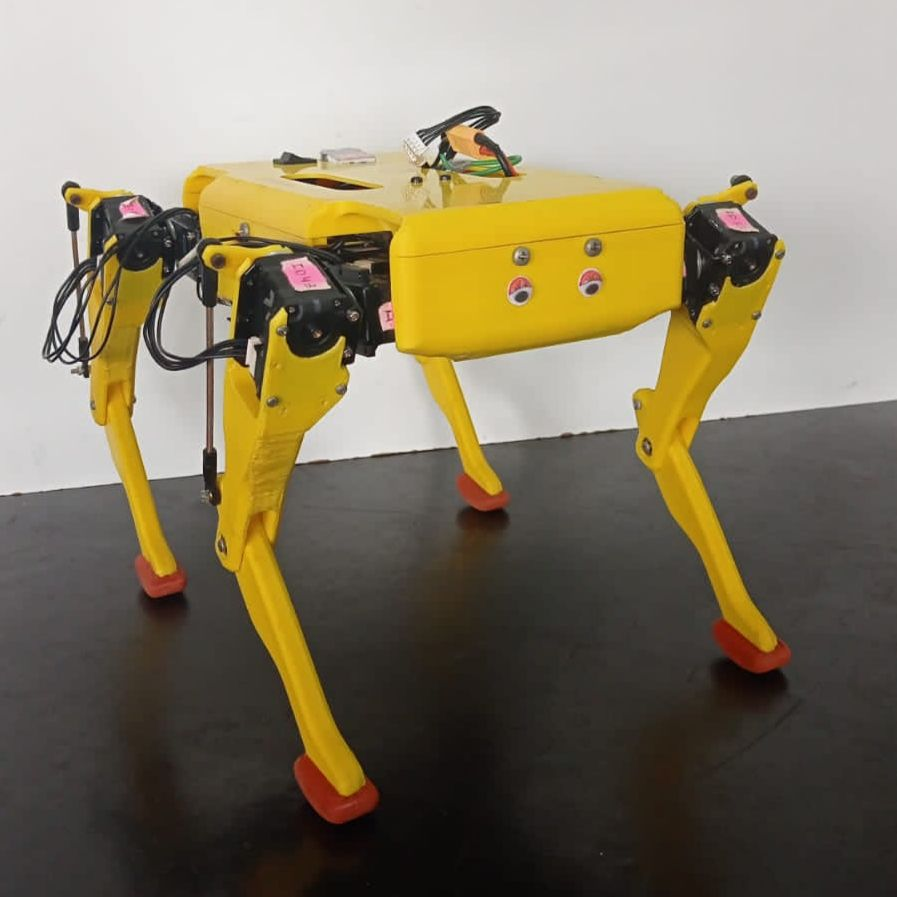
\includegraphics[width=0.4\textwidth]{robot.jpeg}
  \vfill
  \caption{The quadruped robot.}
  \label{fig:robot}
  \vspace{-\baselineskip}
\end{figure}

\subsection{Prototype}

During the prototyping phase, the hardware architecture and physics structure was designed. Following that, the structure of the robot was printed in ABS (Acrylonitrile Butadiene Styrene) and integrated with the hardware components. The robot's actuators are servo motors of the model Dynamixel MX-28, and a Raspberry Pi 4 was chosen as the processing unit. Furthermore, it contains an inertial sensor of the model MPU6050. All the software was developed with the Robot Operating System 2 Humble (ROS 2) \cite{ROS2Humble}.

The robot's structure is mammal-type, which is characterized by the presence of two joints in the sagittal plane, similar to animals such as dogs and horses \cite{Kitano2016}.  The robot's legs follow a configuration called full-elbow, in which the four legs have their lower joints (the tibia joint) oriented backward, as shown in Fig. \ref{fig:robot}. Furthermore, it features 3 degrees of freedom (DoF) per leg, providing the legs with substantial freedom of movement. The robot was designed to favor the mass balance between the body and the robot's legs, that is, the majority of its mass is located in the body or as close to it as possible. Lighter legs can move quickly without significantly changing the center of gravity of the robot, which increases stability and requires less control complexity.  On the other hand, the legs should be strong enough to support the robot's weight and the impact on the ground \cite{Zhong2019}.

The internal components, which include sensors, the processing unit, and the communication interface with the actuators were arranged symmetrically in the robot's body. The actuators (components that contribute to most of the system's mass) were positioned as close as possible to the body. The motor that acts on the tibia joint was placed in the upper part of the femur, to reduce the moment of inertia of the leg, which then required the addition of a transmission system between the engine and the tibia link, consisting of a rigid metal rod with a ball joint at each edge.

\subsection{Gait Planner}

Quadruped robots move according to a gait pattern. The gait implemented for the robot follows the sequence of phases demonstrated in Fig. \ref{fig:trot_pattern}, in which the white rectangles represent the swing phase and the gray rectangles represent the stance phase. During the stance phase, the legs are on the ground and push the robot's body in the desired direction. In the swing phase, the legs are raised and moved to the next support point. The gait pattern illustrated in Fig. \ref{fig:trot_pattern} is called trot and is based on the concept of periodic and symmetrical gaits. The periodic gaits are characterized by the continuous repetition of the movements in the same instants. Symmetry is a characteristic of gaits that move a pair of legs together, leaving and returning to the ground in a synchronized way \cite{de2006quadrupedal}. Although the structure of the robot makes it possible to perform other types of gaits, in this work, only the trot was considered. To reduce the control complexity, a discontinuous gait was adopted, that is, the robot's body moves only when all the legs are on the ground, resulting in intermittent movement. In Fig. \ref{fig:trot_pattern}, it is noticeable that the same pair of diagonal legs always move at the same instant. Between two consecutive swing phases, there is a moment when all legs are in the stance phase, which is when the robot body is displaced in the desired direction of motion.

\begin{figure}[b]
  \vspace{-\baselineskip}
  \centering
  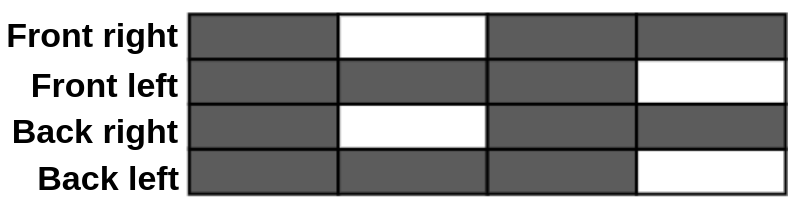
\includegraphics[width=0.45\textwidth]{trot_pattern.png}
  \vfill
  \caption{Gait pattern diagram.}
  \label{fig:trot_pattern}
\end{figure}

For the robot to move according to the adopted gait pattern, there is a gait planner responsible for commanding the robot's legs. The gait planner defines where each foot will step and where the body should move based on the desired velocity of the robot. A trajectory planner calculates the trajectory each foot and body should follow. Then, the gait planner reads, from the stabilization controller, the corrections in pitch and roll angles and applies them before sending the commands to each joint, at a frequency of $\SI{50}{\hertz}$. To convert both trajectories' points and the control efforts into the angles of the joints, a kinematic model is used, which is responsible for mapping the three-dimensional position of one foot to the joints' angles of its respective leg.

\subsection{Trajectory Planner}

The trajectory planner is responsible for calculating the trajectory that each foot must perform. For both the stance and swing phases, a cycloidal curve was adopted. As shown in \cite{Shi2021}, a cycloidal curve can be defined in the three-dimensional space by (\ref{eq:traj_x}) to (\ref{eq:traj_k})
between the points $(x_o, y_o, z_o)$ and $(x_f, y_f, z_f)$ as a function of time $t$, step height $H$, and period $T$.

\begin{equation}
  x = (x_f - x_o) \frac{K - \sin{(K)}}{2 \pi} + x_o
  \label{eq:traj_x}
\end{equation}
\begin{equation}
  y = (y_f - y_o) \frac{K - \sin{(K)}}{2 \pi} + y_o
  \label{eq:traj_y}
\end{equation}
\begin{equation}
  z = H \frac{1 - \cos{(K)}}{2} + z_o
  \label{eq:traj_z}
\end{equation}
\begin{equation}
  K = \frac{2 \pi t}{T}
  \label{eq:traj_k}
\end{equation}

The plot of a cycloidal curve in 3D space is shown in Fig. \ref{fig:traj_space}. The same trajectory is illustrated in Fig. \ref{fig:traj_time} as a function of time. It is noticeable that the curve has a null first derivative when the foot touches the ground, which is favorable to open loop control, since the smoother the landing, the fewer disturbances are caused in the system.

\begin{figure*}[h]
  \centering
  \begin{subfigure}[t]{0.32\textwidth}
    \centering
    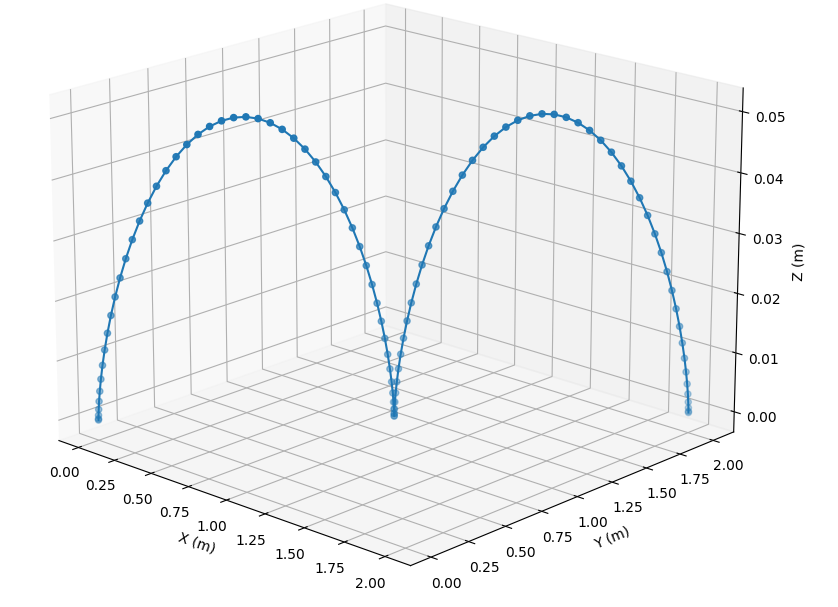
\includegraphics[width=1.0\textwidth]{Cycloid_space.png}
    \caption{The cycloidal curve in 3D space.}
    \label{fig:traj_space}
  \end{subfigure}
  \begin{subfigure}[t]{0.32\textwidth}
    \centering
    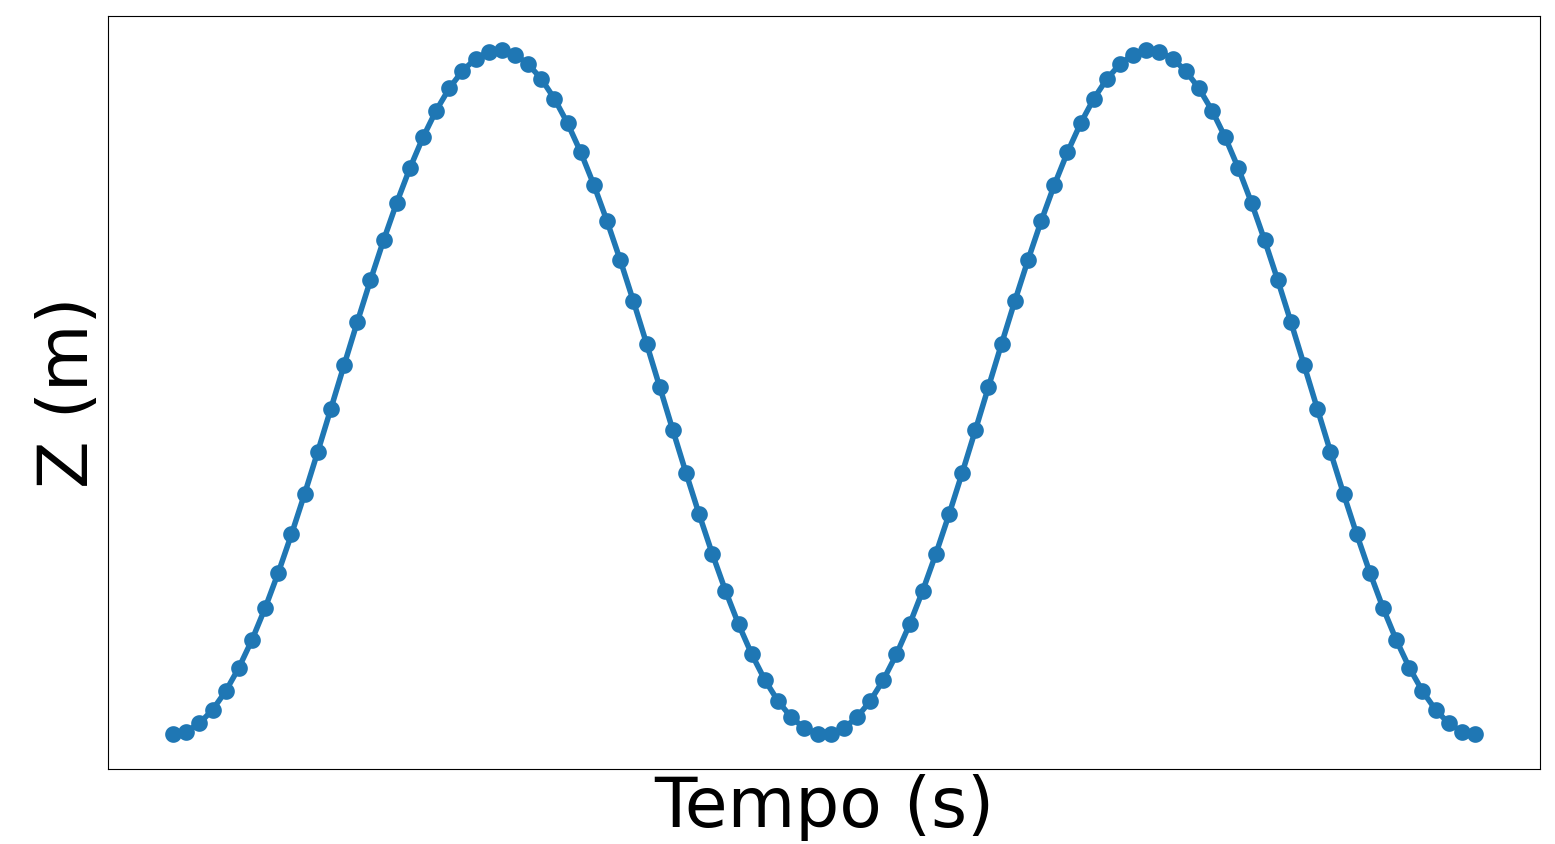
\includegraphics[width=1.0\textwidth]{Cycloid_time.png}
    \caption{The cycloidal curve w.r.t. time.}
    \label{fig:traj_time}
  \end{subfigure}
  \begin{subfigure}[t]{0.32\textwidth}
    \centering
    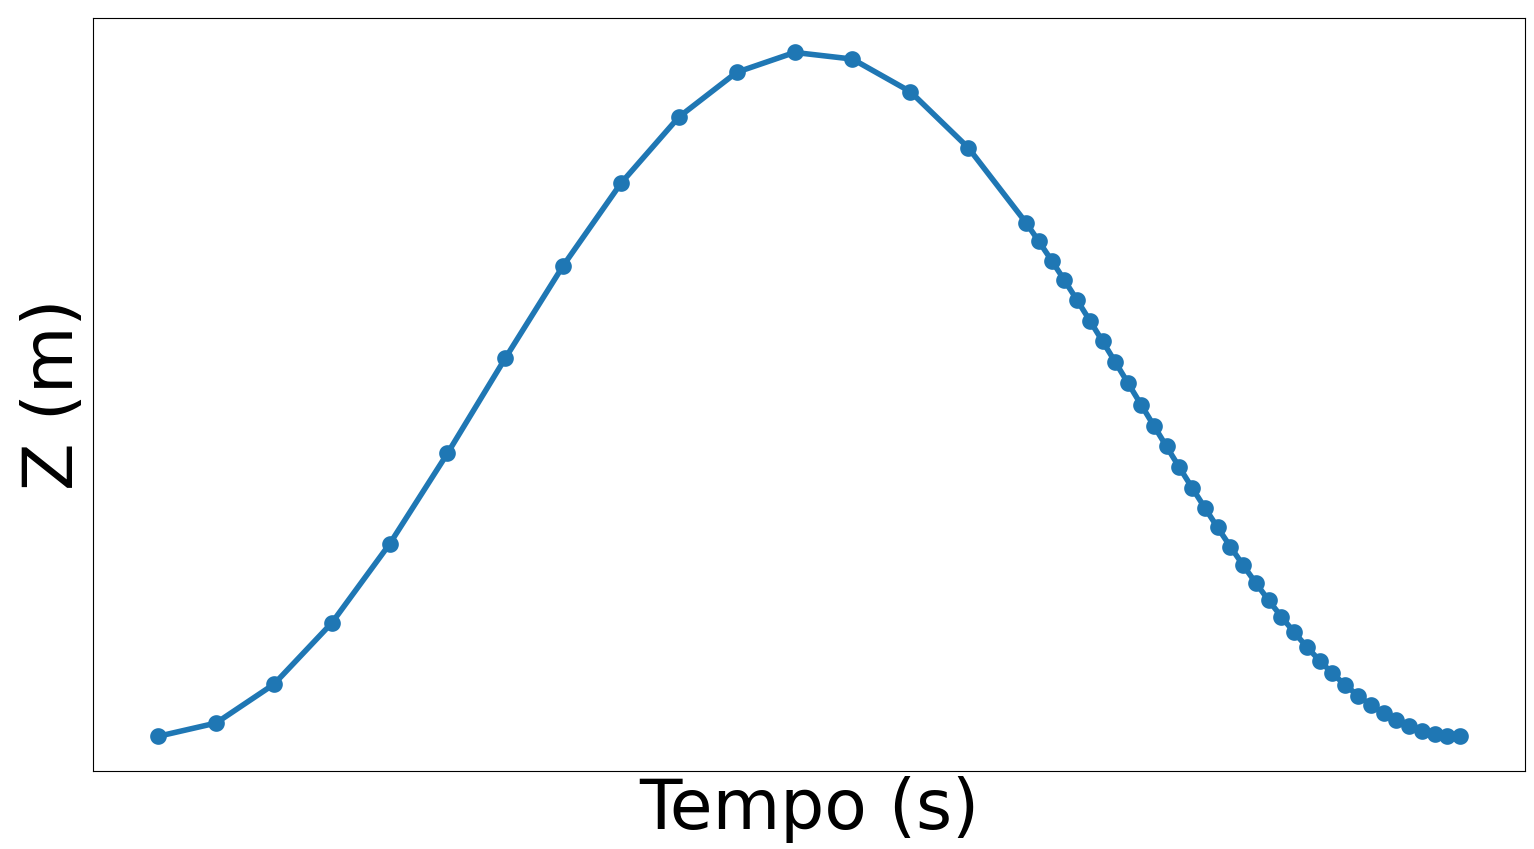
\includegraphics[width=1.0\textwidth]{Cycloid_modified.png}
    \caption{The curve with an uneven distribution of points.}
    \label{fig:traj_time_modified}
  \end{subfigure}
  \vfill
  \caption{Cycloidal trajectories by the trajectory planner.}
  \label{fig:traj_curve}
  \vspace{-\baselineskip}
\end{figure*}

In addition to the step height, the (x, y) translations, and the period, the robot's trajectory planner also considers two parameters to make the landing of the foot even smoother. Since the robot’s actuators are servo motors controlled by position, the torque is proportional to the displacement it must perform between the points of the trajectory. Therefore, the higher the resolution of the trajectory, the smoother the movement. However, the resolution $N$ of the trajectory is fixed, given as a function of the step period and the frequency of the gait planner ($\SI{50}{\hertz}$) $N = 50T$. Thus, the strategy adopted is to distribute the $N$ points unevenly throughout the step period, so that there are more points near the moment the foot lands on the ground and fewer points near the moment the foot takes off. The $P_T$ parameter is a fraction of the total step period, and the $P_N$ is the fraction of the total number of points that should be between $0$ and $P_T \cdot T$. In other words, if $P_T = 0.66$ and $P_N = 0.33$, then 33\% of $N$ will be in the first two-thirds of the period, while the remaining $67\%$ will be in the final one-third. The trajectory, considering these parameters, is illustrated in Fig. \ref{fig:traj_time_modified}.

\subsection{Kinematic Model}
\label{sec:detail_inv_kinematics}

The kinematic model of a quadruped robot describes the relationship between the position of the foot in the three-dimensional space and the rotation of each joint of its corresponding leg. This model is used to solve the forward kinematics, which provides the position $(x, y, z)$ of the foot as a function of the leg joint's angles, and the inverse kinematics, which provides the rotation of each joint to achieve the desired $(x, y, z)$ position of the foot. Moreover, this model can be extended to encompass the kinematics of the quadruped's body.

The package tf2 \cite{tf2}, an available ROS 2 feature that can manage transformations between coordinate axes, was used to solve the robot's forward kinematics, and the inverse kinematics was solved based on geometric analysis. The variables $\theta_1$, $\theta_2$ and $\theta_3$ express the angular position of each leg joint (angles of hip, femur and tibia, respectively), and they can be calculated with the help of \eqref{eq:theta1} to \eqref{eq:B}, as a function of the desired position of the foot w.r.t. to the hip link $(x_{IK}, y_{IK}, z_{IK})$ and the lengths $L_1$, $L_2$ and $L_3$ (Fig. \ref{fig:caramel_tfs}).

\begin{equation}
  \label{eq:theta1}
  \theta_1 = \arctan{(\frac{x_{IK}}{y_{IK}})} - \arctan{(\frac{L_1}{a})}
\end{equation}
\begin{equation}
  \label{eq:theta2}
  \theta_2 = \frac{\pi}{2} - \arctan{(\frac{a}{z_{IK}}}) - \arctan{(\frac{\sqrt{1-A^2}}{A})}
\end{equation}
\begin{equation}
  \label{eq:theta3}
  \theta_3 = \arctan(\frac{\sqrt{1-B^2}}{B})
\end{equation}
\begin{equation}
  \label{eq:a}
  a = \sqrt{x_{IK}^2+y_{IK}^2-L_1^2}
\end{equation}
\begin{equation}
  \label{eq:A}
  A =\frac{a^2+z^2+L_2^2-L_3^2}{2L_2\sqrt{a^2+z_{IK}^2}}
\end{equation}
\begin{equation}
  \label{eq:B}
  B = \frac{a^2+z_{IK}^2-L_2^2-L_3^2}{2L_2L_3}
\end{equation}

\begin{figure}[tb]
  \centering
  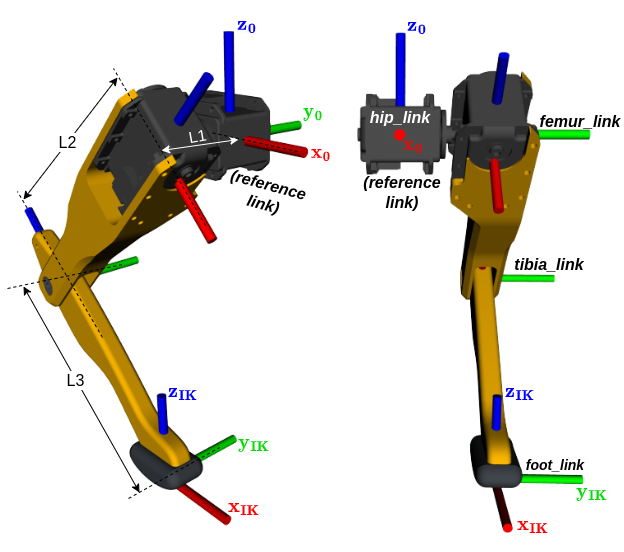
\includegraphics[width=0.4\textwidth]{caramel_tfs.png}
  
  \caption{Links from the robot leg.}
  \label{fig:caramel_tfs}
\end{figure}

These equations are useful for calculating only one foot's position but are insufficient for the robot's body kinematics. For that, a center frame called base\_link (Fig. \ref{fig:caramel_body}) is taken as a reference. The transformation matrix $T_M$ is created with the desired body translations $(x_c, y_c, z_c)$ and rotations $(\alpha, \beta, \gamma)$. The transformations $T_{FR}$, $T_{FL}$, $T_{BL}$ and $T_{BR}$ of each of the four hip\_links with respect to the base\_link are also required.

\begin{figure}[tb]
  \centering
  \vspace{-0.75cm}
  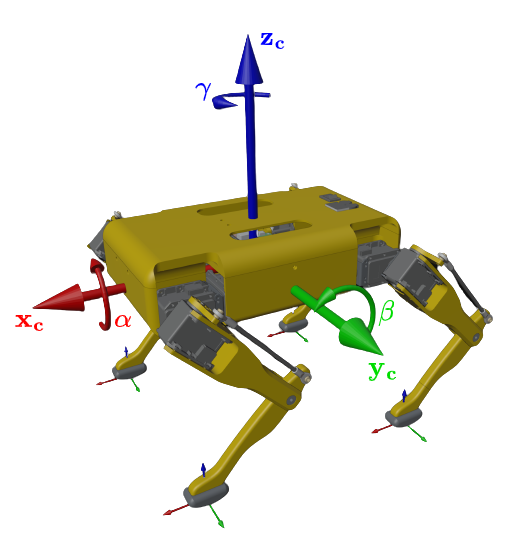
\includegraphics[width=0.35\textwidth]{caramel_body.drawio.png}
  
  \caption{Robot axes in resting position.}
  \label{fig:caramel_body}
  \vspace{-1.3\baselineskip}
\end{figure}

The calculation of the joints' angles of each leg is then performed using as inputs the values resulting from each of the transformations, according to (\ref{eq:xyzik}). While $[x, y, z, 1]^\top$ in the right-hand side of (\ref{eq:xyzik}) represents the foot position relative to the base\_link, $[x_{IK}, y_{IK}, z_{IK}, 1]^\top$ on the left-hand side represents the same position relative to the leg's hip\_link, which can be used as input in equations (\ref{eq:theta1}) to (\ref{eq:B}). 

\begin{equation}
  \label{eq:xyzik}
  \begin{bmatrix}
    x_{IK} \\
    y_{IK} \\
    z_{IK} \\
    1
  \end{bmatrix}= (T_M.T_{FR})^{-1}.
  \begin{bmatrix}
    x \\
    y \\
    z \\
    1
  \end{bmatrix}
\end{equation}

The same calculation can be done for the other legs, by substituting $T_{FR}$ by $T_{FL}$, $T_{BL}$, or $T_{BR}$ in \eqref{eq:xyzik}. In this way, \eqref{eq:xyzik} allows computing the angles $\theta_1$, $\theta_2$ and $\theta_3$ of each leg from the desired position of each foot and the desired translations and rotations of the body, using the same frame as reference (base\_link). It means one can control all the six DoFs of the body together with the positions of the feet at the same time.

\subsection{Control Subsystem}

The control subsystem of the robot is composed of two main components: the joints' controllers, and the body's stabilization controller. The joints' controllers are the built-in Dynamixel position PID controllers, and they control each joint of the robot independently. Meanwhile, the body's stabilization controller is responsible for controlling the pitch and roll angles of the robot \cite{Shi2021, StanfordPupper}, maintaining it at 0 degrees.  

The stabilization controller is formed by two PID controllers: for the roll and pitch rotation of the robot's body. They act independently, stabilizing the rotation in each axis simultaneously. Both controllers are identical and were implemented following the block diagram in Fig. \ref{fig:pid} (the output of the "IMU Sensor" block is either roll or pitch).

\begin{figure}[b]
  \vspace{-\baselineskip}
  \centering
  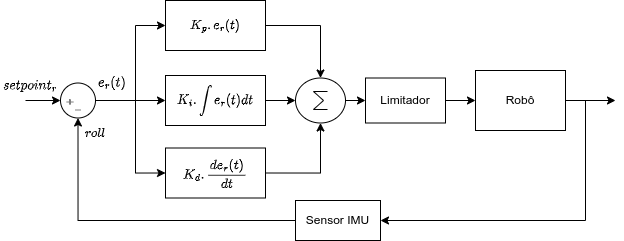
\includegraphics[width=0.48\textwidth]{PID.drawio.png}
  \caption{Designed PID controller.}
  \label{fig:pid}
\end{figure}

The IMU sensor is responsible for measuring the rotation of the robot's body, providing feedback on the system's outputs. The limiter was added to avoid body rotations that exceed the limits of the joints.

\section{Results} \label{results}

To assess the robot's locomotion performance, three experiments were conducted. The first experiment aimed to test the trajectory tracking of one single leg in a no-load scenario, a more ideal case. The second experiment evaluated the robot's capability of following a forward velocity setpoint and the amplitude of its body oscillations' while walking in a straight line, i.e. stability, in flat and uneven terrain. Therefore, in the first experiment, the fundamental functionality of performing one gait step with one leg was tested, while in the second the system was submitted to a realistic operation scenario where the gait planner must manage the movement of all legs and the body. The third experiment was similar to the second but focused on the yaw motion of the robot and was performed only on uneven terrain.

For the first experiment, the robot's body was supported on a platform so that its leg would not touch the floor, lowering the load applied to the motors. The experiment consisted of sending gait trajectories to a single leg and evaluating how precise the leg could follow it. The trajectories were cycloidal curves with a height of 0.05 cm, a period of 0.5 seconds and a resolution of 25 equally distributed points ($P_T = P_N = 1.0$). The distances in the (x, y) directions were (5.0, 3.0) and (3.0, 5.0) cm, and, for each distance pair, 30 samples were collected. Table \ref{tab:trajetoria} shows the average and standard deviation of the time taken to complete the trajectory, the height, and the distance reached by the leg in the (x, y) direction. Test 1 refers to the trajectories of the first distance pair and Test 2 to the second. Fig. \ref{fig:grafico_trajetoria_xyz} shows the z-axis (height) tracking of one sample, where the blue curve is the trajectory commands (in meters) over time (in seconds) and the red curve is the trajectory performed by the foot.

\begin{table}[!b]
  \vspace{-\baselineskip}
  \centering
  \caption{Results of the gait trajectory tracking experiment.}
  \scalebox{1.3}{
  \begin{tabular}{ccc}
    \hline
    \textbf{Test} & \textbf{1}      & \textbf{2}  \\
    \hline
    $\bar{time} (s)$         & 0.557  & 0.557 \\
    \hline
    $\sigma_{time} (s)$       & 0.008  & 0.008 \\
    \hline
    $\bar{z}_{max} (cm)$       & 4.760  & 4.755 \\      
    \hline
    $\sigma_{z_{max}} (cm)$    & 0.023  & 0.028 \\
    \hline
    $\bar{x}_{final} (cm)$     & 5.034  & 3.024 \\
    \hline
    $\sigma_{x_{final}} (cm)$  & 0.009  & 0.013 \\
    \hline
    $\bar{y}_{final} (cm)$     & 2.924  & 4.915 \\      
    \hline
    $\sigma_{y_{final}} (cm)$  & 0.013  & 0.004 \\      
    \hline   
  \end{tabular}
  }
  \label{tab:trajetoria}
\end{table}

\begin{figure}[!b]
  \centering
  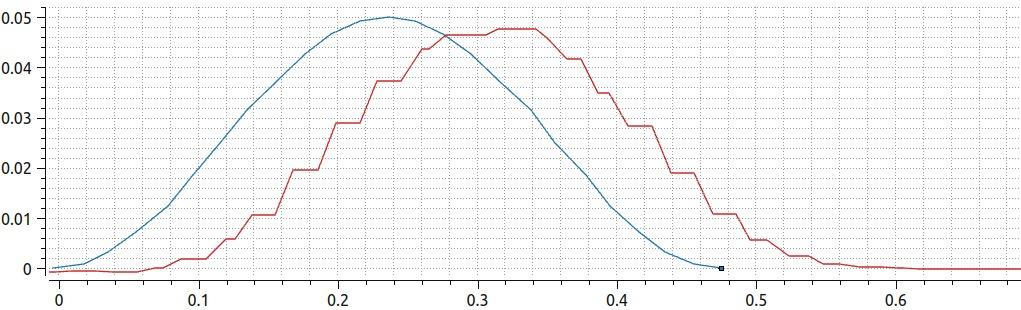
\includegraphics[width=0.48\textwidth]{grafico_trajetoria_z.png}
  \caption{Trajectory executed by the foot.}
  \label{fig:grafico_trajetoria_xyz}
  \vspace{-\baselineskip}
\end{figure}

It is noticeable that there was a delay of approximately 57 milliseconds in the execution time and that the final height was off by approximately 0.25 centimeters in both tests. To confirm that the system's performance during Test 1 and 2 was similar, i.e. the difference in (x, y) distance did not affect the overall performance, two ANOVA \cite{cano2012six} tests were conducted comparing the execution time and gait height distributions of both tests. Before the ANOVA, the outliers of these distributions were removed and the Shapiro-Wilk \cite{leotti2005comparaccao} test was used to check the data normality. The result of the latter was a p-value greater than 0.05 for all distributions, which indicates that they followed a normal curve. The ANOVA tests were, then, conducted and showed a p-value of 0.7212 for the execution time comparison and 0.5070 for the gait height comparison, which means that de difference in the (x, y) distance did not affect the trajectory tracking performance. In addition to that, the final average error for x and y was less than 0.1 centimeters and the standard deviation was small, meaning the gait distance was followed correctly and that this result was consistent throughout all samples.

For the second experiment, the robot should walk in a straight line of 1.5 meters in both flat and uneven terrain, with and without the stabilization controller, totalizing four tests. The flat terrain consisted of a cement floor and the uneven terrain, a ground formed by small loose stones. Both are illustrated in Fig. \ref{fig:terreno_plano} and \ref{fig:terreno_uneven}, respectively.

\begin{figure}[tb]
  \centering
  \begin{subfigure}[htbp]{0.24\textwidth}
    \centering
    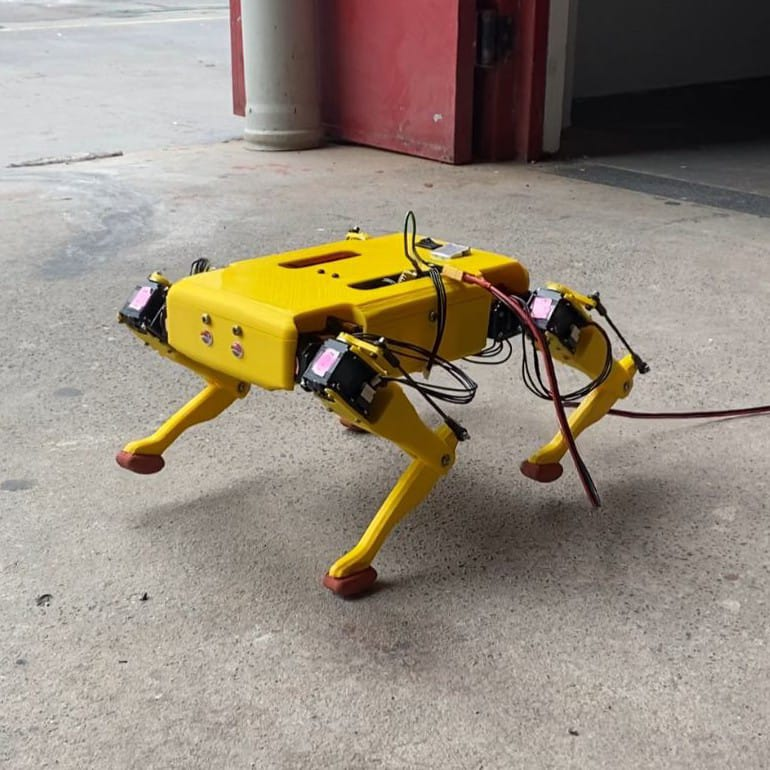
\includegraphics[width=1.0\textwidth]{terreno_plano.jpeg}
    \caption{Flat.}
    \label{fig:terreno_plano}
  \end{subfigure}
  \begin{subfigure}[htbp]{0.24\textwidth}
    \centering
    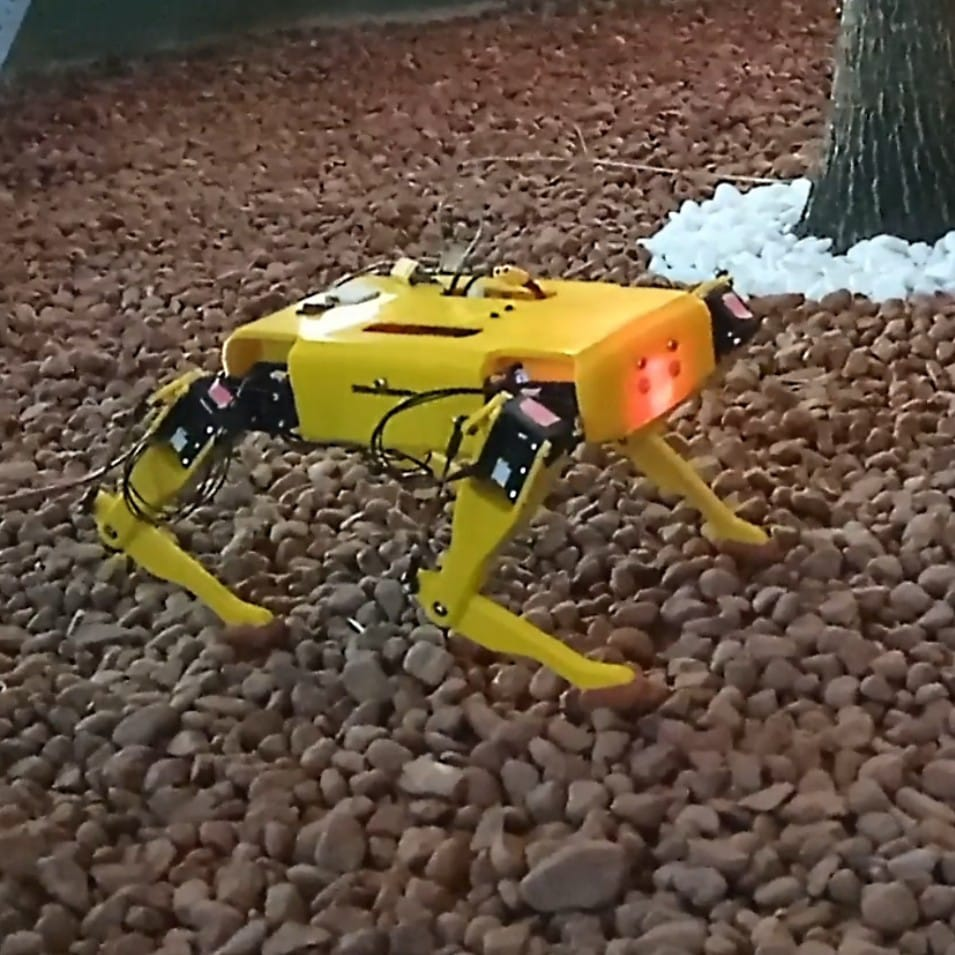
\includegraphics[width=1.0\textwidth]{terreno_irregular.jpeg}
    \caption{Uneven.}
    \label{fig:terreno_uneven}
  \end{subfigure}
  \vfill
  \caption{Terrains used for the experiment.}
  \label{fig:terrenos}
  \vspace{-\baselineskip}
\end{figure}

For each test, the robot received a forward velocity command of 0.05 m/s. Its mean velocity, as well as its pitch and roll oscillation, were recorded. The mean velocity was calculated based on the time it took to travel 1.5 meters and the oscillation is the difference between the maximum and minimum readings of the IMU. The calculated velocity was compared to the desired velocity sent to the robot and the oscillation data was analyzed statistically following the same procedure of the trajectory tracking experiment.

For all the tests, the robot's gait settings consisted of a height of 5 centimeters, a period of 0.5 seconds, a resolution of 25 points, $P_T$ = 0.66, and $P_N$ = 0.33. For each test type, 10 samples were collected.

Table \ref{tab:vel_stab} summarizes the collected results. The robot did not reach a velocity of 0.05 m/s in any test. This result is due to steady state errors in the final position of each leg during the swing phase: the legs could not reach the desired (x, y) position required during the gait period, to maintain the desired velocity. The fact that the final position of one foot is a function of its motors' final orientation indicates that the motors did not reach their desired orientation. And since no significant errors were noted during the previous experiment (a more ideal situation), they were perhaps caused by a lack of power from the motors, which were not able to support the robot's weight appropriately while walking.

\begin{table}[!h]
  \centering
  \caption{Velocity and stability results.}
  \scalebox{1.3}{
  \begin{tabular}{ccccc}
    \hline
    \textbf{Test}              & \textbf{1}   & \textbf{2}  & \textbf{3}   & \textbf{4}   \\ \hline
    Ter.                       & Flat         & Flat        & Uneven       & Uneven       \\ \hline
    \begin{tabular}[c]{@{}c@{}}S. C. \end{tabular} & No           & Yes         & No           & Yes          \\ \hline
    \begin{tabular}[c]{@{}c@{}}Vel. \\ $(cm/s)$ \end{tabular} & 2.15         & 3.68        & 2.03         & 2.39         \\ \hline
    \begin{tabular}[c]{@{}c@{}} $\sigma_{Vel}$  \\ $(cm/s)$ \end{tabular} & 0.040        & 0.075       & 0.016        & 0.047        \\ \hline
    \begin{tabular}[c]{@{}c@{}} $\Delta_{Roll}$ \end{tabular} & 12.59\degree & 8.81\degree & 13.37\degree & 11.13\degree \\\hline
    \begin{tabular}[c]{@{}c@{}} $\sigma_{Roll}$ \end{tabular} & 2.54\degree  & 2.36\degree & 0.78\degree  & 1.47\degree  \\ \hline
    \begin{tabular}[c]{@{}c@{}} $\Delta_{Pitch}$ \end{tabular} & 11.55\degree & 8.31\degree & 15.19\degree & 12.09\degree \\ \hline
    \begin{tabular}[c]{@{}c@{}} $\sigma_{Pitch}$ \end{tabular} & 1.89\degree  & 2.63\degree & 1.44\degree  & 1.66\degree  \\ \hline
  \end{tabular}
  }
  \label{tab:vel_stab}
  % \vspace{-\baselineskip}
\end{table}

In addition to the velocity results, the pitch and roll oscillations were compared to determine whether or not the stabilization controller lowered the robot's body oscillation. The Shapiro-Wilk test was applied to the data from all the tests, after removing outliers, and every test returned a p-value greater than 0.05, which indicates that the distributions followed a normal curve. The ANOVA was, then, applied to compare the roll and pitch oscillations from tests 1 and 2 (flat terrain). The same process was applied to the tests 3 and 4 as well. The ANOVA revealed that the roll and pitch distributions of the tests with and without stabilization control were significantly different. Table \ref{tab:vel_stab} shows that the mean value of the oscillations in both axes of the tests with stabilization control was less than the mean value of the tests without it, indicating that the stabilization controller lowered the robot's body oscillations in both terrain types. Fig. \ref{fig:imu_test} better pictures the data distribution. Despite the more scattered distribution, 3 out of 4 of the tests with stabilization control had its third quartile less than the first quartile of the distribution without the controller for the same terrain type, demonstrating that the controller lowered the oscillations in at least 75\% of the collected test samples.
\vspace{0.1\baselineskip}

\begin{figure}[!tb]
  \centering
  \begin{subfigure}[t]{0.49\textwidth}
    \centering
    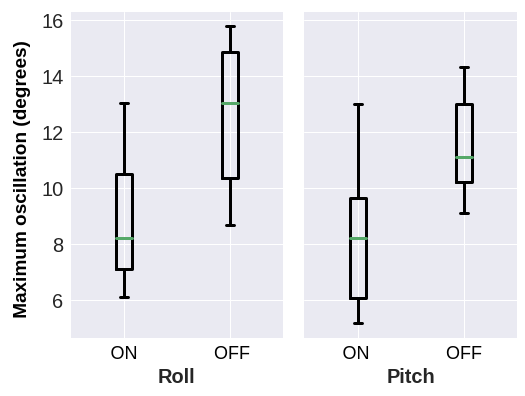
\includegraphics[width=1.0\textwidth]{plane_boxplot.png}
    \caption{Flat terrain.}
    \label{fig:imu_test_plane}
  \end{subfigure}
  \begin{subfigure}[t]{0.49\textwidth}
    \centering
    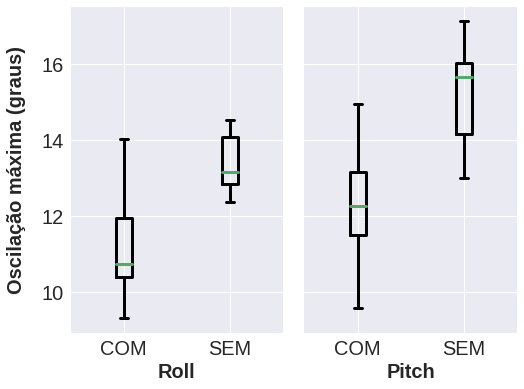
\includegraphics[width=1.0\textwidth]{irregular_boxplot.png}
    \caption{Uneven terrain.}
    \label{fig:imu_test_irregular}
  \end{subfigure}
  \caption{Robot body's oscillation in both terrains.}
  \label{fig:imu_test}
  % \vspace{-1.5\baselineskip}
\end{figure}

Finally, in the third experiment, the robot was placed in the same uneven terrain and was commanded to follow a yaw motion of 0.25 rad/s. The experiment was conducted until the robot had completed a full rotation around its z-axis. Again, the time, roll oscillation and pitch oscillation were recorded along 10 samples with and without the stabilization controller. 

Table \ref{tab:ang_vel_stab} summarizes the collected results. The robot did not reach the angular velocity setpoint of 0.25 rad/s but maintained a steady 0.19 rad/s in both tests with a very low standard deviation, suggesting no significant differences. The body rotation analysis was also performed as before. The Shapiro-Wilk test presented a p-value greater than 0.05, which led to the application of the ANOVA test. The ANOVA test between the roll oscillation distributions with and without the stabilization controller resulted in a p-value of approximately 0.5, supporting the thesis that the controller did not affect the yaw motion significantly. The ANOVA test for the pitch oscillation, on the other hand, shows that the pitch oscillation was slightly bigger with the stabilization controller, which explains a much lower p-value, around 0.07. This result, though different from the previous two, still indicates no significant changes in the stabilization controller while the robot performs a yaw movement.

\begin{table}[!h]
  \centering
  \caption{Angular velocity and stability results.}
  \scalebox{1.3}{
  \begin{tabular}{ccc}
    \hline
    \textbf{Test}              & \textbf{1}   & \textbf{2}   \\ \hline
    Ter.                       & Uneven       & Uneven       \\ \hline
    \begin{tabular}[c]{@{}c@{}}S. C. \end{tabular} & No           & Yes          \\ \hline
    \begin{tabular}[c]{@{}c@{}}Angular vel. \\ $(rad/s)$ \end{tabular} & 0.19         & 0.19         \\ \hline
    \begin{tabular}[c]{@{}c@{}} $\sigma_{Ang. Vel.}$  \\ $(rad/s)$ \end{tabular} & 0.006        & 0.007        \\ \hline
    \begin{tabular}[c]{@{}c@{}} $\Delta_{Roll}$ \end{tabular} & 16.16\degree & 16.84\degree \\\hline
    \begin{tabular}[c]{@{}c@{}} $\sigma_{Roll}$ \end{tabular} & 1.88\degree  & 2.6\degree  \\ \hline
    \begin{tabular}[c]{@{}c@{}} $\Delta_{Pitch}$ \end{tabular} & 11.79\degree & 12.89\degree \\ \hline
    \begin{tabular}[c]{@{}c@{}} $\sigma_{Pitch}$ \end{tabular} & 1.05\degree  & 1.41\degree  \\ \hline
  \end{tabular}
  }
  \label{tab:ang_vel_stab}
  % \vspace{-\baselineskip}
\end{table}

% \begin{figure}[!tb]
%   \centering
%   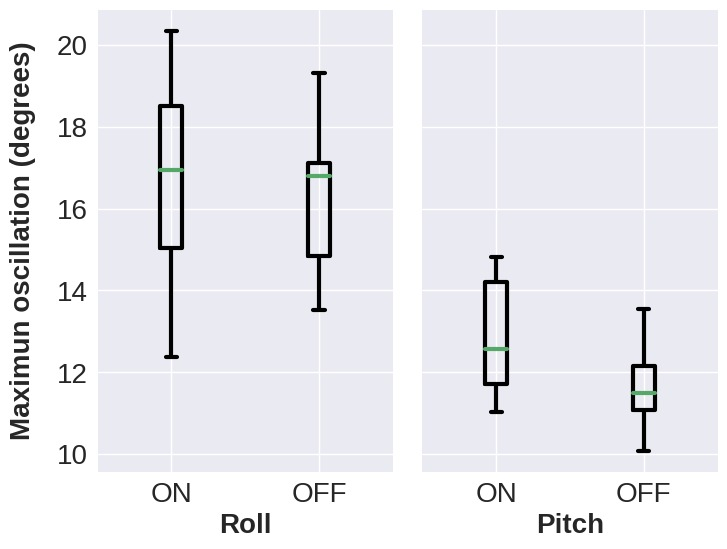
\includegraphics[width=0.5\textwidth]{ang_vel_boxplot.png}
%   \caption{Robot body's oscillation during yaw motion.}
%   \label{fig:ang_vel_boxplot}
%   % \vspace{-1.5\baselineskip}
% \end{figure}

\section{Conclusion} \label{conclusion}

This paper addressed the design, prototyping and testing of a quadruped robot. Three experiments were held to assess the robot's walking performance. The results showed that the robot did not reach the desired velocity in any of the tests. This was due to errors during the gait's swing phase, which indicates that the motors were unable to support the robot's weight while walking. These errors were not compensated, because the gait's trajectory tracking is open-loop (only the individual joint's controllers are closed-loop). In addition to that, it was possible to conclude that the implemented stabilization controller was able to lower the robot's body oscillations in pitch and roll while walking in a straight line on both flat and uneven terrains, but did not affect the yaw motion of the quadruped on uneven terrain.

Reviewing the robot's actuators is recommended for future work. Perhaps a model with more torque is required for more precise control performance.

The robot's project is open source and is available on GitHub \cite{CaramelRepo}. A demonstration video is also available in \url{https://youtu.be/d0BPT8uhiSc}.

\section*{Acknowledgment}

We would like to express our sincere gratitude to our advisors MSc. Marco Reis and MSc. Paulo Andrade, and to the Centro Universitário SENAI CIMATEC for their valuable support and contributions to this project. We also extend our thanks to all those who have provided assistance and support throughout this research endeavor. %TODO

% \section*{References}

% Please number citations consecutively within brackets \cite{b1}. The
% sentence punctuation follows the bracket \cite{b2}. Refer simply to the reference
% number, as in \cite{b3}---do not use ``Ref. \cite{b3}'' or ``reference \cite{b3}'' except at
% the beginning of a sentence: ``Reference \cite{b3} was the first $\ldots$''

% Number footnotes separately in superscripts. Place the actual footnote at
% the bottom of the column in which it was cited. Do not put footnotes in the
% abstract or reference list. Use letters for table footnotes.

% Unless there are six authors or more give all authors' names; do not use
% ``et al.''. Papers that have not been published, even if they have been
% submitted for publication, should be cited as ``unpublished'' \cite{b4}. Papers
% that have been accepted for publication should be cited as ``in press'' \cite{b5}.
% Capitalize only the first word in a paper title, except for proper nouns and
% element symbols.

% For papers published in translation journals, please give the English
% citation first, followed by the original foreign-language citation \cite{b6}.
%----------------------------------------------------------
\bibliographystyle{IEEEtran}
\bibliography{Bibliography}
%CRITICAL: do not change the above two lines!!!
%----------------------------------------------------------

% \begin{thebibliography}{00}
%   \bibitem{X.134} X. Zhang, L. Lang, J. Wang, and H. Ma, ‘The quadruped robot locomotion based on force control’, Proceedings of the 2015 27th Chinese Control and Decision Conference, CCDC 2015, pp. 5440–5445, 2015.
%   \bibitem{ROS2Humble} S. Macenski, T. Foote, B. Gerkey, C. Lalancette, and W. Woodall, ‘Robot Operating System 2: Design, architecture, and uses in the wild’, Science Robotics, vol. 7, no. 66, p. eabm6074, 2022.
%   \bibitem{Kitano2016} S. Kitano, S. Hirose, A. Horigome, and G. Endo, ‘TITAN-XIII: sprawling-type quadruped robot with ability of fast and energy-efficient walking’, ROBOMECH Journal, vol. 3, pp. 1–16, 2016.
%   \bibitem{Zhong2019} Y. Zhong, R. Wang, H. Feng, and Y. Chen, ‘Analysis and research of quadruped robot’s legs: A comprehensive review’, International Journal of Advanced Robotic Systems, vol. 16, 3 2019.
%   \bibitem{de2006quadrupedal} P. G. De Santos, E. Garcia, and J. Estremera, ‘Quadrupedal locomotion: an introduction to the control of four-legged robots’, vol. 1. Springer, 2006.
%   \bibitem{Shi2021} Y. Shi, S. Li, M. Guo, Y. Yang, D. Xia, and X. Luo, ‘Structural design, simulation and experiment of quadruped robot’, Applied Sciences (Switzerland), vol. 11, 2021.
%   \bibitem{StanfordQuadruped} N. Kau, A. Z. Schultz, and M. Bowers, ‘Stanford Quadruped’. Github.com. https://github.com/stanfordroboticsclub/StanfordQuadruped. (Accessed Jun. 13, 2023).
%   \bibitem{JointTrajectory} ros2\_control Development Team. ‘Joint Trajectory Controller’. Control.ros.org. https://control.ros.org/foxy/doc/ros2\_controllers/joint\_trajectory\_contro
%   ller/doc/userdoc.html. (Accessed Jun. 13, 2023).
%   \bibitem{cano2012six} E. L. Cano, J. M. Moguerza, and A. Redchuk, Six sigma with R: statistical engineering for process improvement, vol. 36. Springer Science \& Business Media, 2012.
%   \bibitem{leotti2005comparaccao} V. B. Leotti, A. R. Birck, and J. Riboldi, ‘Comparação dos Testes de Aderência à Normalidade Kolmogorov-smirnov, Anderson-Darling, Cramer--Von Mises e Shapiro-Wilk por Simulação’, Anais do 11\textordmasculine Simpósio de Estatística Aplicada à Experimentação Agronômica, 2005.
%   \bibitem{CaramelRepo} B. S. de Alencar, F. M. S. M. Barreto, and L. L. Souza (2022), ‘Caramel’. Github.com. https://github.com/Brazilian-Institute-of-Robotics/bir-black-mouth. (Accessed Jun. 13, 2023).

%   % 14   STANFORD Quadruped. Dispon ́ıvel em:〈https://github.com/stanfordroboticsclub/StanfordQuadruped〉. Acesso: 24 de nov de 2022.15   DIY hobby servos quadruped robot.Dispon ́ıvel em:〈https://hackaday.io/project/171456-diy-hobby-servos-quadruped-robot〉.Acesso: 24 de nov de 2022.
%   % 15   DIY hobby servos quadruped robot.Dispon ́ıvel em:〈https://hackaday.io/project/171456-diy-hobby-servos-quadruped-robot〉.Acesso: 24 de nov de 2022.
%   % 17   NOTSPOT robot simulation. Dispon ́ıvelem:〈https://github.com/lnotspotl/notspot_sim_cpp〉. Acesso: 24 de nov de 2022.

%   % \bibitem{b1} G. Eason, B. Noble, and I. N. Sneddon, ``On certain integrals of Lipschitz-Hankel type involving products of Bessel functions,'' Phil. Trans. Roy. Soc. London, vol. A247, pp. 529--551, April 1955.
%   % \bibitem{b2} J. Clerk Maxwell, A Treatise on Electricity and Magnetism, 3rd ed., vol. 2. Oxford: Clarendon, 1892, pp.68--73.
%   % \bibitem{b3} I. S. Jacobs and C. P. Bean, ``Fine particles, thin films and exchange anisotropy,'' in Magnetism, vol. III, G. T. Rado and H. Suhl, Eds. New York: Academic, 1963, pp. 271--350.
%   % \bibitem{b4} K. Elissa, ``Title of paper if known,'' unpublished.
%   % \bibitem{b5} R. Nicole, ``Title of paper with only first word capitalized,'' J. Name Stand. Abbrev., in press.
%   % \bibitem{b6} Y. Yorozu, M. Hirano, K. Oka, and Y. Tagawa, ``Electron spectroscopy studies on magneto-optical media and plastic substrate interface,'' IEEE Transl. J. Magn. Japan, vol. 2, pp. 740--741, August 1987 [Digests 9th Annual Conf. Magnetics Japan, p. 301, 1982].
%   % \bibitem{b7} M. Young, The Technical Writer's Handbook. Mill Valley, CA: University Science, 1989.
% \end{thebibliography}
% \vspace{12pt}
% \color{red}
% IEEE conference templates contain guidance text for composing and formatting conference papers. Please ensure that all template text is removed from your conference paper prior to submission to the conference. Failure to remove the template text from your paper may result in your paper not being published.

\end{document}
